\documentclass[12pt]{article}
\usepackage[utf8]{inputenc}
\usepackage{lipsum}
\usepackage{amssymb}
\usepackage{setspace}
\usepackage{indentfirst}
\usepackage{setspace}
\usepackage{blindtext}
\usepackage{titlesec}
\usepackage{slashed}
\usepackage{tensor}
\usepackage{array}
\usepackage[T1]{fontenc}
\usepackage{xspace}
\newcommand{\Poincare}{Poincar\'e\xspace}
\newcommand{\Lubanski}{Luba\'nski\xspace}
\newcommand{\Kahler}{K$\ddot{\text{a}}$hler\xspace}
\usepackage{graphicx}
\usepackage{geometry}
\geometry{margin=1in}
\usepackage{setspace}
\graphicspath{ {./images/} }
\doublespacing
\usepackage{physics,mathtools,amsmath}


\usepackage{dsfont}
\usepackage{float}
\usepackage{subfig}
\usepackage{siunitx}

\title{Johnson Noise}
\author{\AE ther Zhou, Vivian Liao }
\date{March 2023}

\begin{document}

\maketitle

\begin{abstract}
\quad Johnson noise is the electrical noise fundamental to the resistance of a circuit that is generated by the thermodynamic property of the conducted circuit and depends on only the temperature and conductivity of the system. In this lab, we studied the relation between the RMS voltage and resistances under specific temperature. By measuring the thermal noises of a series of shorted resistors with a filtered amplifier, we estimated absolute zero temperature to be $-286 \pm 16 \,\si{^\circ C}$, in agreement with the accepted value $-273.15\,\si{^\circ C}$. We also calculated the Boltzmann constant by controlling the temperature of the resistors. However, our calculated value $(1.665\pm 0.094)\times 10^{-23}\,\si{J\cdot K^{-1}}$ deviates from the accepted value $1.381\times 10^{-23}\,\si{J\cdot K^{-1}}$ by $21\%$. A possible cause for this discrepancy is the variation in background noise, which we will explore further in the Error Analysis section. 

\end{abstract}

\newpage

\section{Introduction}

\quad Johnson noise is the electrical noise that is fundamental to the resistance of a circuit. It is generated by the thermodynamic property of the conducted circuit and is present in all electrical circuits, which is one of the main limiting factors in many areas. In particular, it causes a noise floor below that is not possible to proceed, which thus limits the sensitivity of equipment such as radio receivers.

As stated in Nyquist's paper, the factor that determines the amplitude of the noise is the sum of the energy in the normal modes of electrical oscillation. According to Nyquist's theorem, the RMS voltage $V_j$ evolved in the circuit is given by
\begin{gather}
d{V_j}^{2}=4Rk_BTdf
\label{eqn:nyquist's theorem}
\end{gather}
where $R$ is the resistor, $T$ is the temperature, and $df$ is the frequency interval.

However, the system we used for measurement has its characteristic impedance due to its capacitance $C$ forming a low pass filter. It modifies the resistance $R$ and gives a frequency dependent resistance $R_f$ as expressed by $R_f=\frac{R}{1+(2\pi fCR)^2}$.
% \begin{gather}
% R_f=\frac{R}{1+(2\pi fCR)^2}
% \label{eqn:modified resistance}
% \end{gather}
Also, the measurement system of a low noise pre-amplifier and filter creates an amplification of the voltage depending on the Johnson voltage $dV=[g(f)]^2dV_j$.
% \begin{gather}
% dV=[g(f)]^2dV_j
% \label{eqn:modified voltage}
% \end{gather}
Substitute the modified resistance and the amplified voltage into Eqn.~\ref{eqn:nyquist's theorem} and integrate over, we arrive at
\begin{gather}
V^2=4Rk_BTG
\label{eqn:nyquist's theorem final}
\end{gather}
where $G$ is the band gain of the system expressed as $G=\int_{0}^{\infty} \frac{[g(f)]^2}{1+(2\pi fCR)^2} \,df$.
% \begin{gather}
% G=\int_{0}^{\infty} \frac{[g(f)]^2}{1+(2\pi fCR)^2} \,df
% \label{eqn:band gain}
% \end{gather}

 Eqn.~\ref{eqn:nyquist's theorem final} implies that this thermal noise depends only on the temperature and conductivity of the system. It increases with temperature and depends on constant $k_B$. With measurements of the noise over different resistances and under different temperatures, we can get experimental values for the absolute zero temperature and the Boltzmann constant $k_B$.

\section{Experimental Methods}

\subsection{Equipment}
\quad The general overview of our setup is that the noise source is amplified and filtered by the pre-amplifier and filter, and then sent into a spectral analyzer, which converts the electric signal into frequency domain via Fast Fourier Transformation (FFT). The noise sources are a series of resistors with resistances ranging from 1 k$\Omega$ to 100 k$\Omega$, and a white noise generator is used for the calculation of the system gain. The setup is shown in Fig.~\ref{fig:setup} below.
\begin{center}
    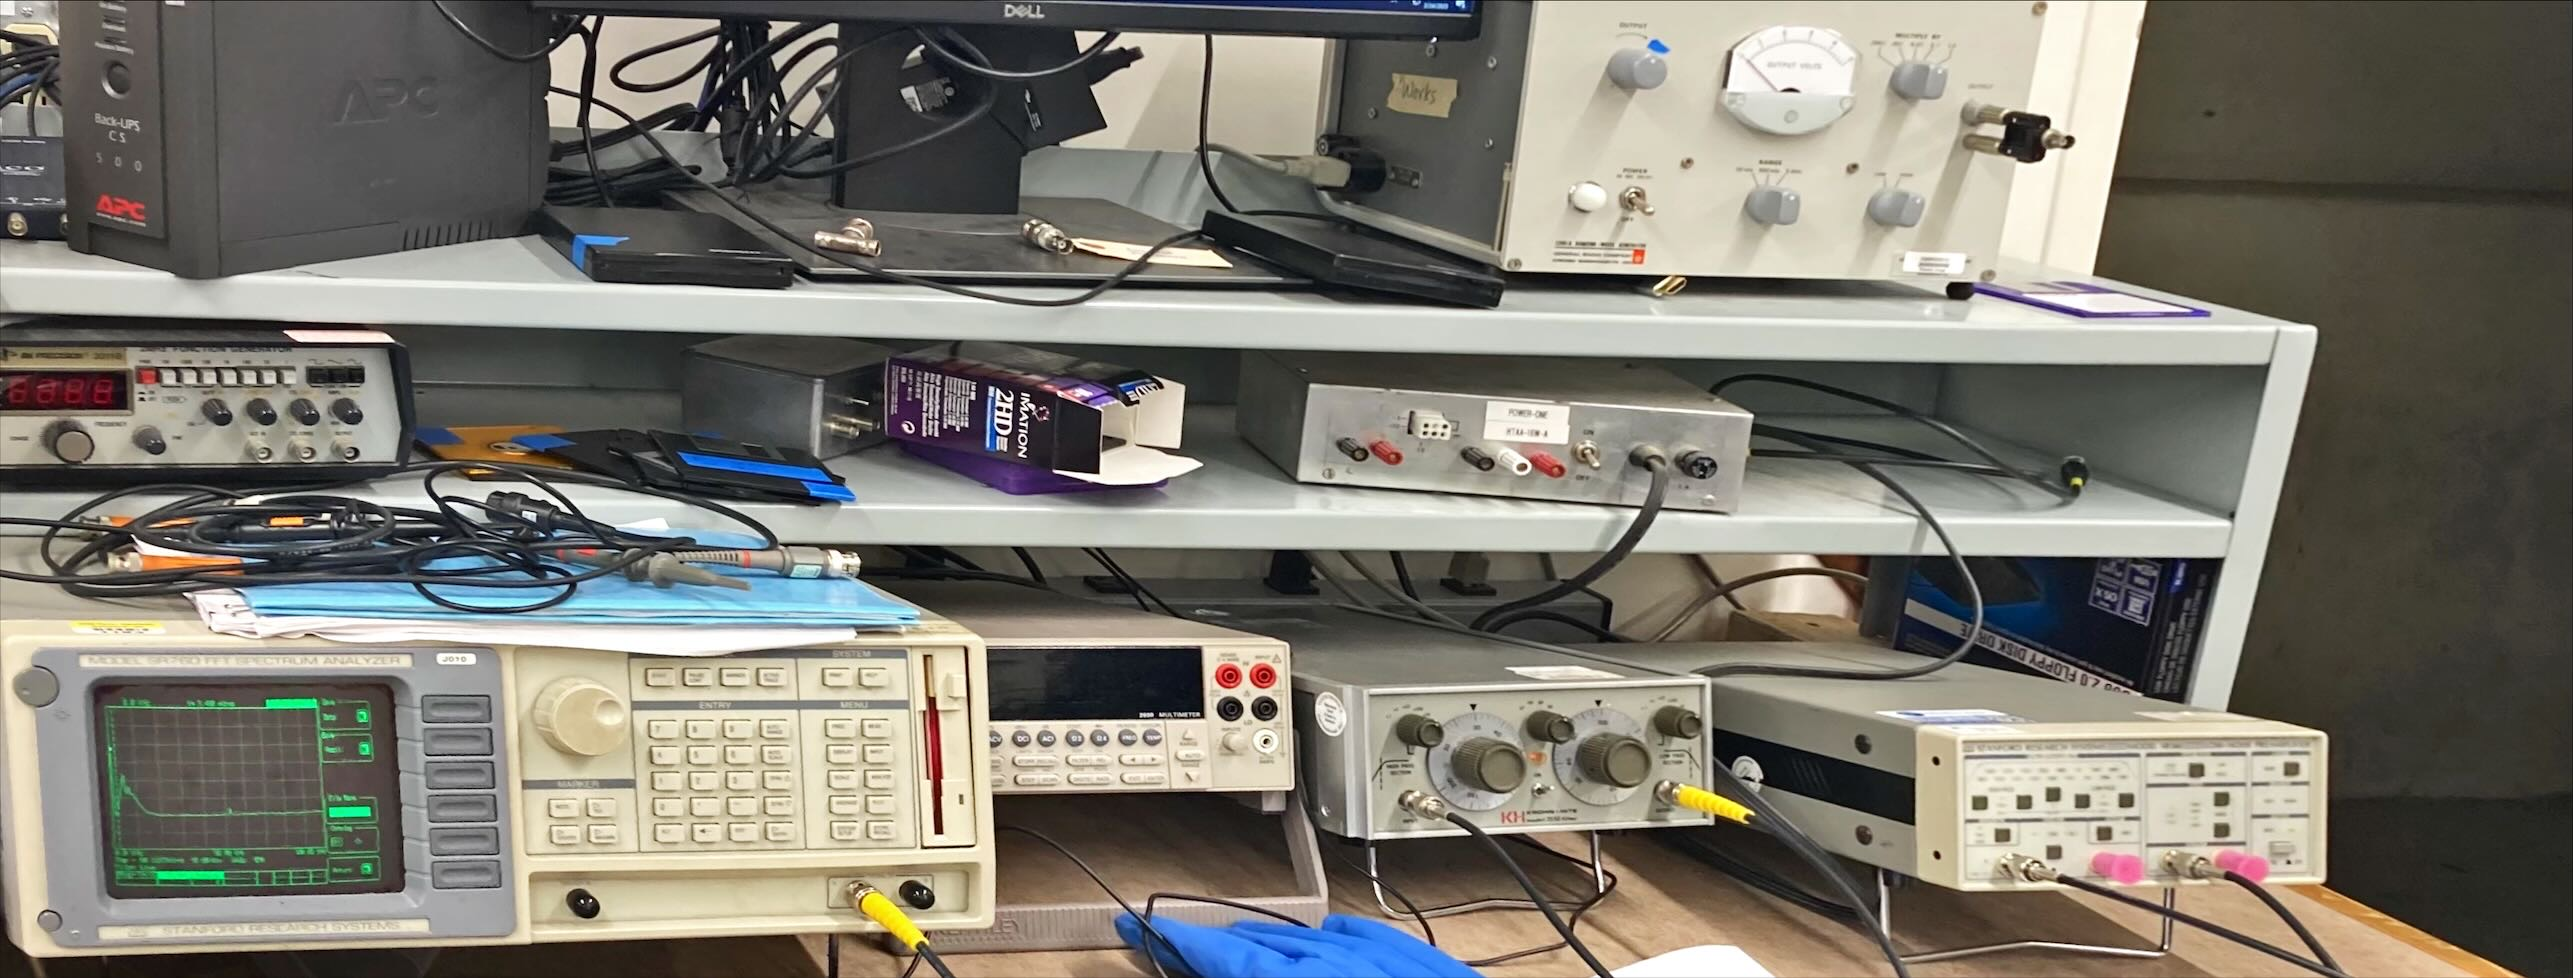
\includegraphics[width= 0.8\textwidth]{images/setup_photo.jpg}
    \captionof{figure}{The setup of the experimental equipment.}
    \label{fig:setup}
\end{center}


\subsection{Steps and Measurement}
\quad First, we calculated the system gain by measuring the noise generated by the white noise generator. The effective gain of a system of electronics as a function of frequency is given as
\begin{gather}
g(f)=\frac{V_{out}(f)}{V_{in}(f)}
\label{eqn:gain}
\end{gather}
where $V_{out}$ is the output voltage of the amplifier-filter chain, and $V_{in}$ is the voltage of the white noise itself. Thus, two measurements are done, one with the noise input directly into the spectral analyzer, and the other with noise amplified and filtered first and input into analyzer. The pre-amplifier is set to AC coupling with low noise gain mode and a gain of 500. The filter cutoff is set to be 3k and 10k Hz for high-pass and low-pass respectively. The output voltage of the noise generator is set right below the overload voltage of the pre-amplifier.

Second, a series of resistors are used as the noise sources. The signal is sent through the amplifier-filter chain with the same setup and input into spectral analyzer. Measurements under two temperatures are conducted, one under room temperature $T=20$ $^\circ$C, and the other at the boiling point of Liquid Nitrogen, which is about $T=-195.79$ $^\circ$C or 77 K.

\section{Raw Data}
% - calibrated the equipment with random noise generator (need plot for g(f))
% - plug in different test resistors (need plot for V(f))

\quad Table~\ref{table:Vrms} listed the band RMS voltage (the total voltage within a specific bandwidth) over the frequency band from 3 kHz to 10 kHz for a series of resistors under two different temperatures. The plotting for RMS voltage under room temperature is shown in FIG.~\ref{fig:raw data room temperature}, and the plotting at Liquid Nitrogen boiling point is shown in FIG.~\ref{fig:raw data liquid nitrogen} below.    In the figures, different colored symbols represent measurements for different resistors. The x-axis is the frequency in range $0-25$ kHz, and the y-axis is the RMS voltage measured and transformed by the spectral analyzer. When limited to frequency bandwidth from 0 to around 15 kHz, the voltage spectra has a nearly Gaussian amplitude distribution. To specify, although listed on the table, the short resistor data are not plotted in the figures.

\quad Also, due to the high precision of the spectral analyzer, our measurement error for $V_{rms}$ is $0.02\%$ of its value, so the $1$-$\sigma$ error bar is difficult to be identified in the following plots (Fig.~\ref{fig:raw data room temperature} \& \ref{fig:raw data liquid nitrogen}).  
\begin{center}
    %\renewcommand{\arraystretch}{1.3}
    \centering
    \begin{tabular}{| l | c | c |}
    \hline
    R [k$\Omega$] & $V_{rms,~20^\circ C}$ [mV] & $V_{rms,~-195.79^\circ C}$ [mV]\\
    \hline
    \hline
    1 & 1.318 & 1.097\\
    10 & 3.281 & 2.065\\
    20 & 4.569 & 2.615\\
    35.2 & 5.878 & 3.329 \\
    48.7 & 6.804 & 3.895\\
    100 & 9.021 & 4.967\\
    short & 0.9291 & 0.9589 \\
    \hline
    $\frac{\delta R}{R} = 1\%$& $\frac{\delta V_{rms}}{V_{rms}} = 0.02\%$&$\frac{\delta V_{rms}}{V_{rms}} = 0.02\%$ \\
    \hline
    \end{tabular}
    \captionof{table}{Raw data of the band RMS voltage over the frequency band from 3 kHz to 10 kHz of different resistors under two different temperatures, $T=20~^\circ$C and $T=-195.79~^\circ$C.} \label{table:Vrms}
\end{center}

\begin{center}
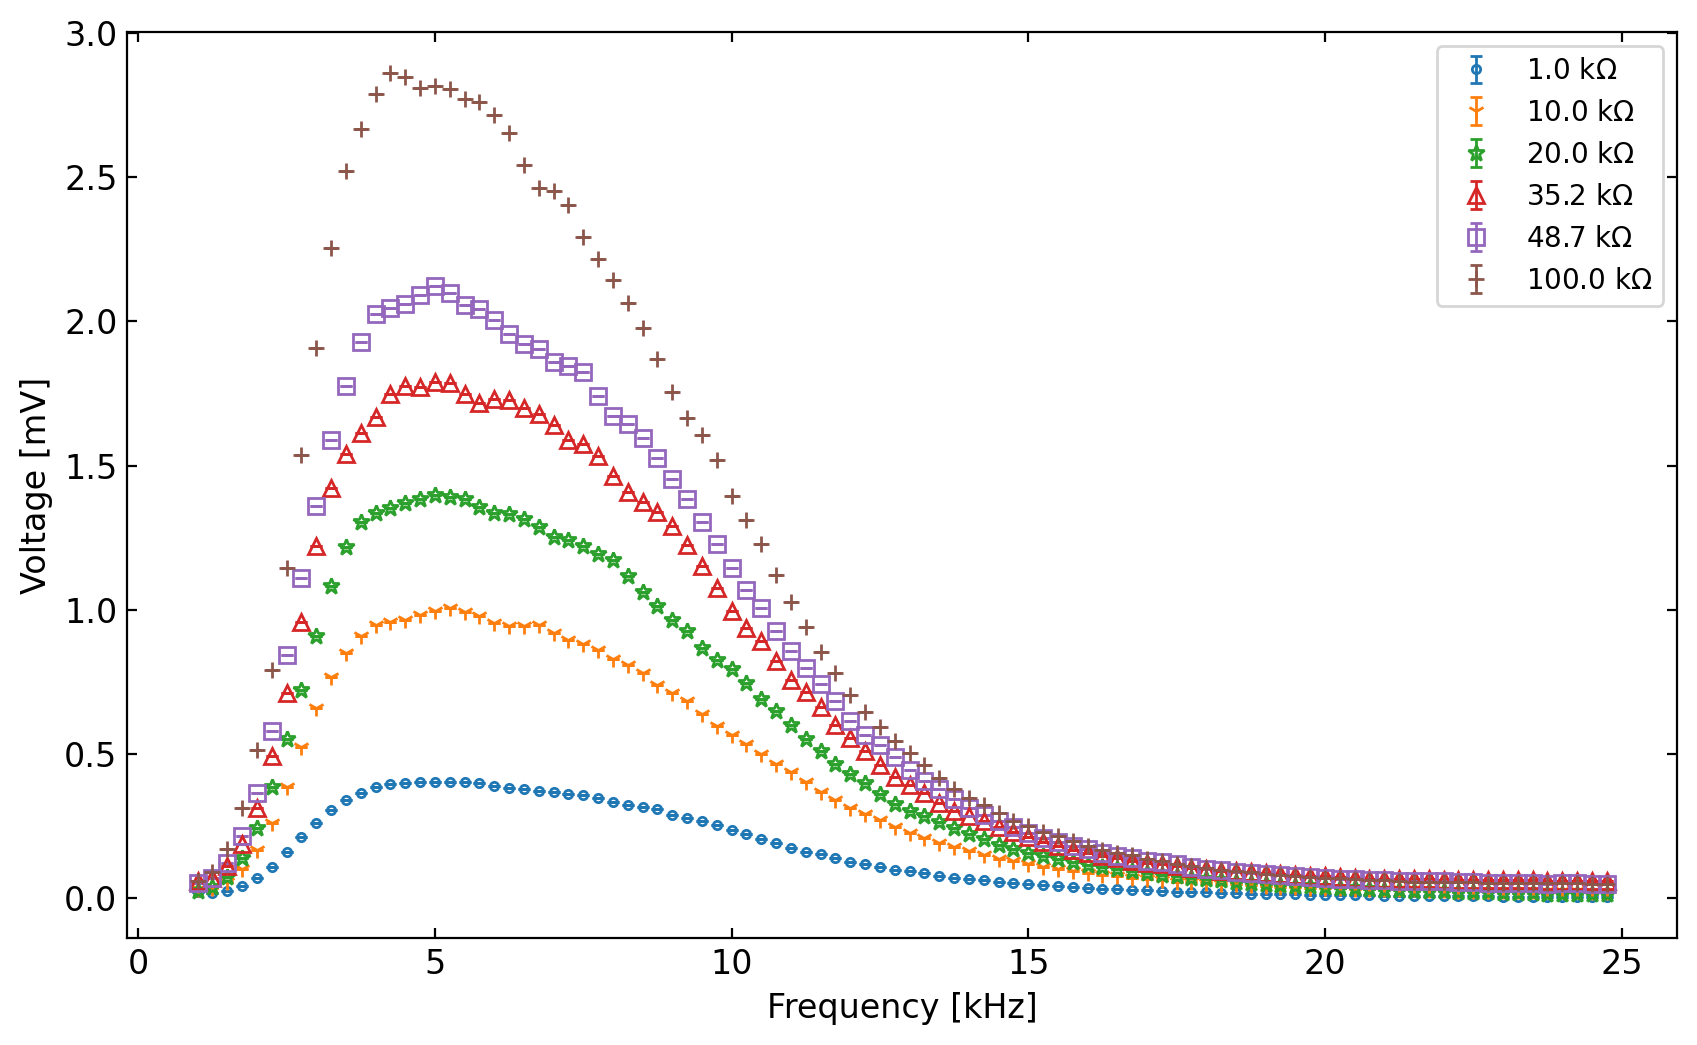
\includegraphics[width = 0.8\textwidth]{images/room_raw.png}
    \captionof{figure}{Raw Data of the RMS voltage of different resistors under room temperature $T=20~^\circ$C. Different colored symbols represent the data point of different resistances. Error bars are presented for each data point.}
    \label{fig:raw data room temperature}
\end{center}

\begin{center}
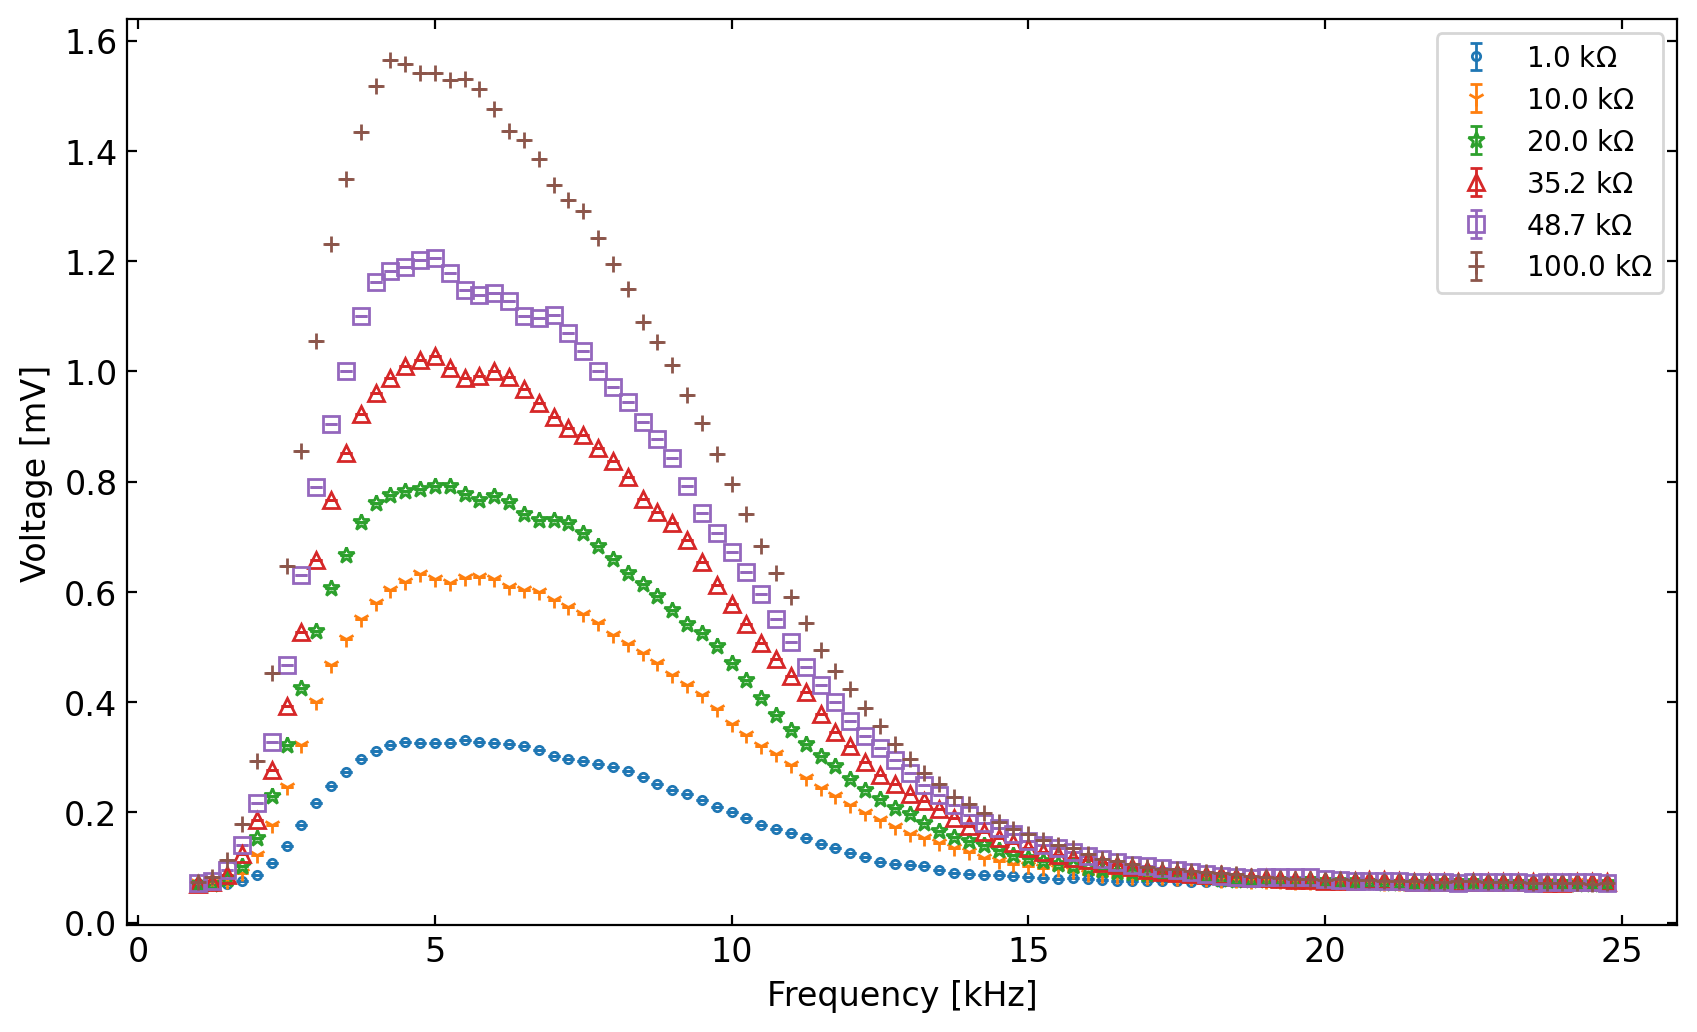
\includegraphics[width = 0.8\textwidth]{images/nitro_raw.png}
    \captionof{figure}{Raw Data of the RMS voltage of different resistors under boiling point of liquid nitrogen $T=-195.79~^\circ$C or 77 K. Different colored symbols represent the data point of different resistances. Error bars are presented for each data point.}
    \label{fig:raw data liquid nitrogen}
\end{center}

\quad We calculated the gain function using Eqn.~\ref{eqn:gain}, and fitted a Gaussian distribution to the data within the 3-10 kHz band (See Fig.~\ref{fig:gauss_fit}). 

\begin{center}
    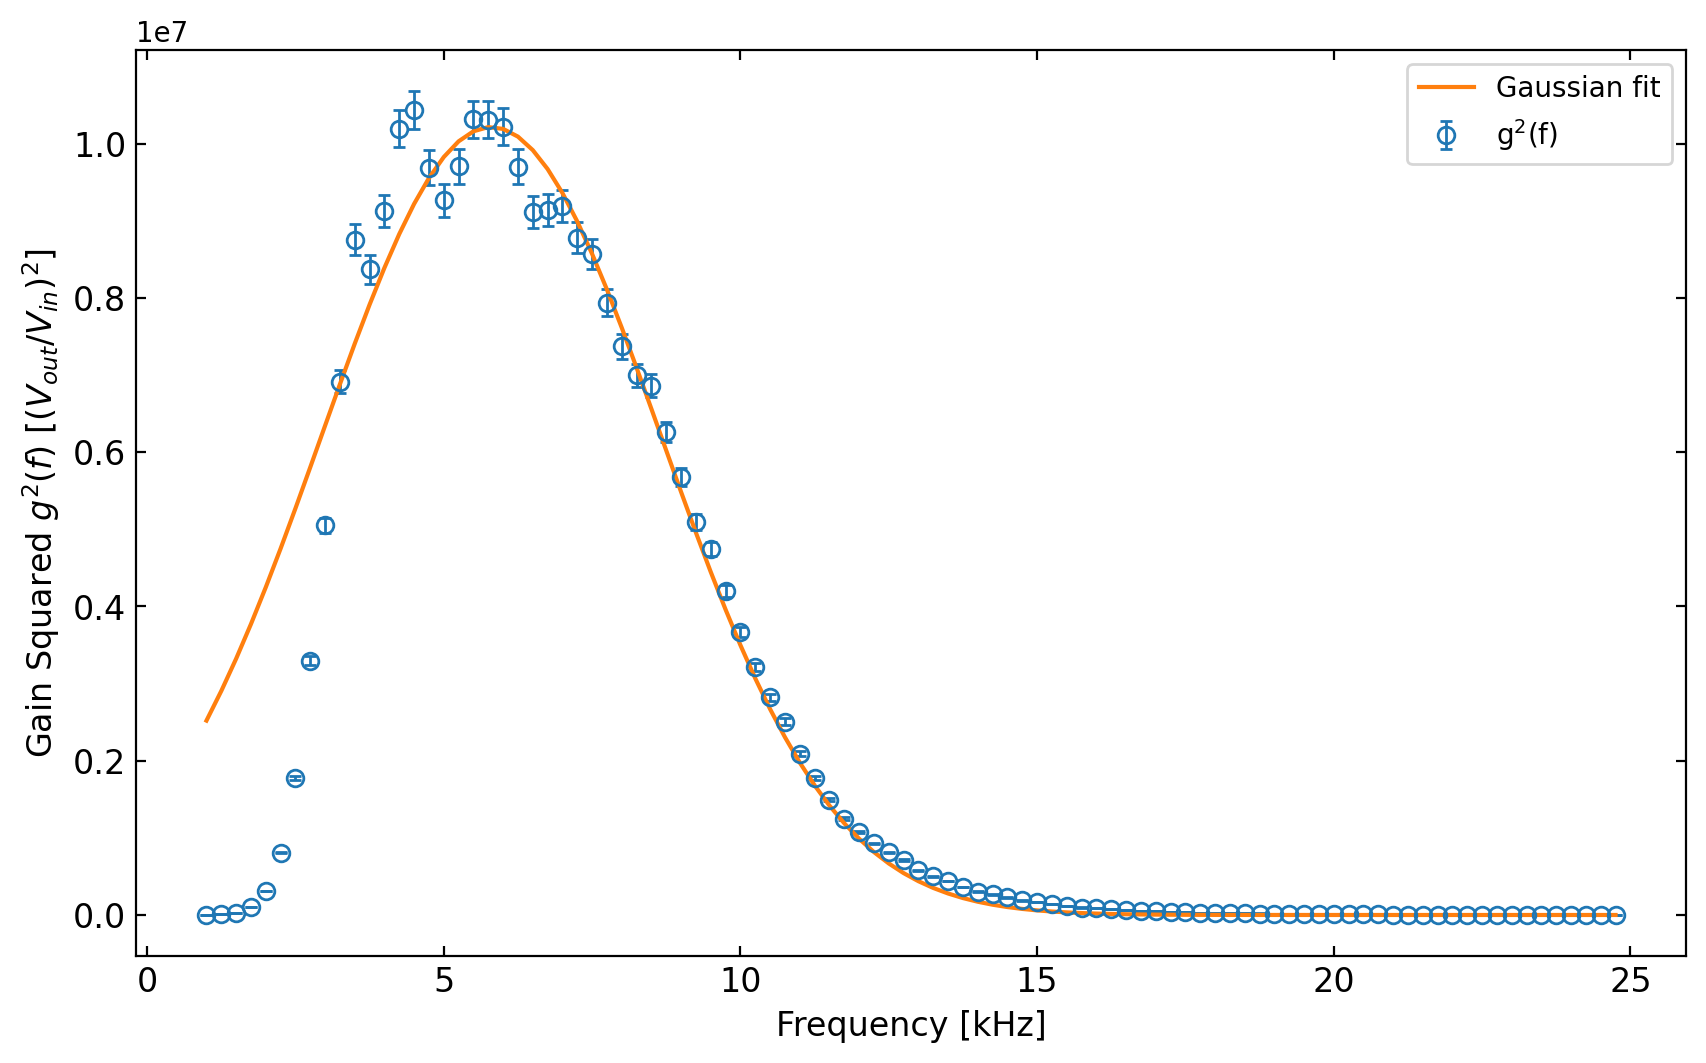
\includegraphics[width = 0.8\textwidth]{images/gauss_gain.png}
    \captionof{figure}{Fitted gain function using the signal from white noise generator. Since $g(f)$ is independent with the signal sources, We will use this to infer the actual magnitude of Johnson noise. We only care about the region between 3 kHz and 10 kHz.}\label{fig:gauss_fit}
\end{center}

\section{Results}

\subsection{Absolute Zero Estimation}
\quad According to Eqn.~\ref{eqn:nyquist's theorem final}, to extract the temperature $T$, we need to perform a linear fit of $\frac{V^2}{4k_BG}$ against $R$. The resulting slope:
\begin{equation}
    \text{slope} = T = \frac{V^2}{4k_BGR} \label{eqn:room_temp}
\end{equation}


Using python scipy.curve\_fit, we manage to extracted the slope $306$ K (See Fig.~\ref{fig:roomTemp}), with a $5\%$ uncertainty. Combined with the room temperature we measured using a thermometer, $20 \pm 1 \,\si{.^\circ C}$, we can estimate the absolute zero: $-286 \pm 16\,\si{.^\circ C}$. And our estimation is in agreement with the accepted value of absolute zero, $-273.15\,\si{.^\circ C}$.

\begin{center}
    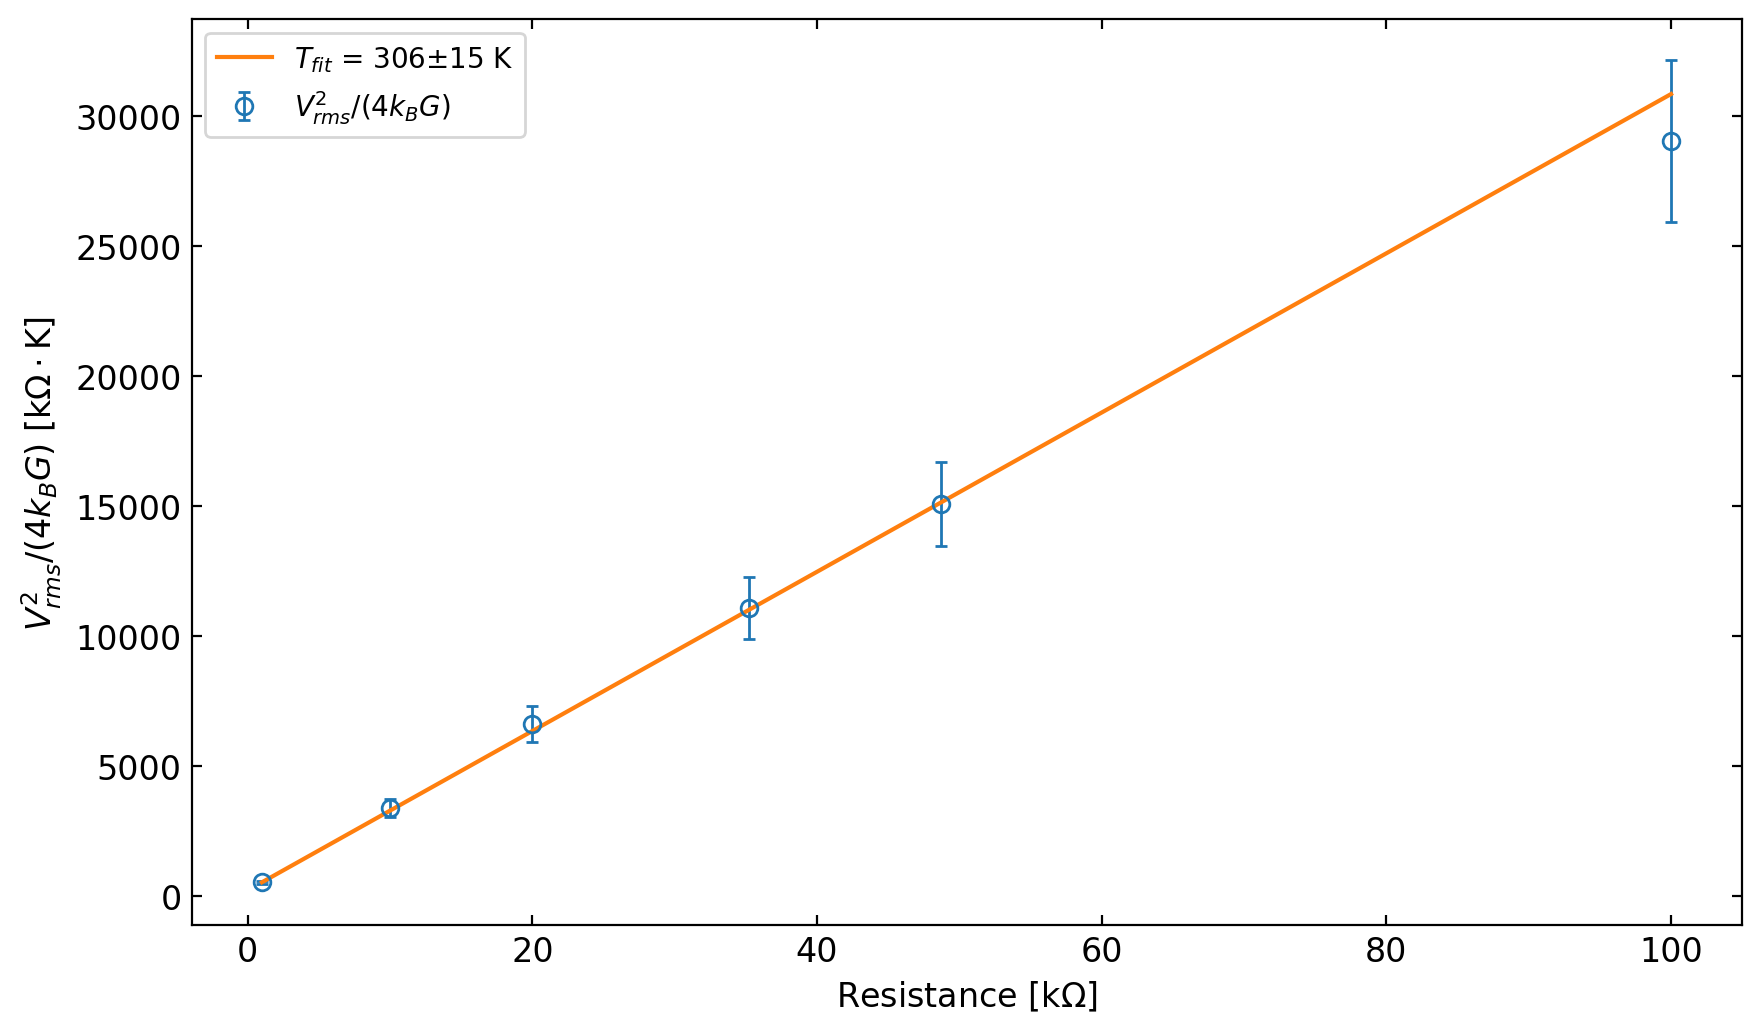
\includegraphics[width=0.8\textwidth]{images/room_fit.png}
    \captionof{figure}{\textbf{Analyzed Plot} - At room temperature ($20 \pm 1 \,\si{.^\circ C}$), we measured Johnson noise of six different resistors, and we performed a line fit based on ratio $V^2_{rms}/(4k_B G)$ versus Resistance. From this we can estimate temperature in Kelvin (proportional to slope) and its uncertainty.}
    \label{fig:roomTemp}
\end{center}


\subsection{Thermodynamic Constant $k_B$ Estimation}
\quad Again according to Eqn.~\ref{eqn:nyquist's theorem final}, to extract the Boltzmann constant $k_B$, we need to perform a linear fit of $\frac{V^2}{4TG}$ against $R$. The resulting slope:
\begin{equation}
    \text{slope} = k_B = \frac{V^2}{4TGR} \label{eqn:nitro_boil}
\end{equation}

By submerging testing resistors into boiling liquid nitrogen, we cooled them to temperature $T = 77\,\si{K}$. 
Using python scipy.curve\_fit, we manage to extracted the slope $(1.665\pm 0.094)\times 10^{-23}\, \si{J\cdot K^{-1}}$  (See Fig.~\ref{fig:boltzConst}), which does not agree with the accepted value of thermodynamic constant, $1.381\times 10^{-23}\,\si{.J \cdot K^{-1}}$.

\begin{center}
    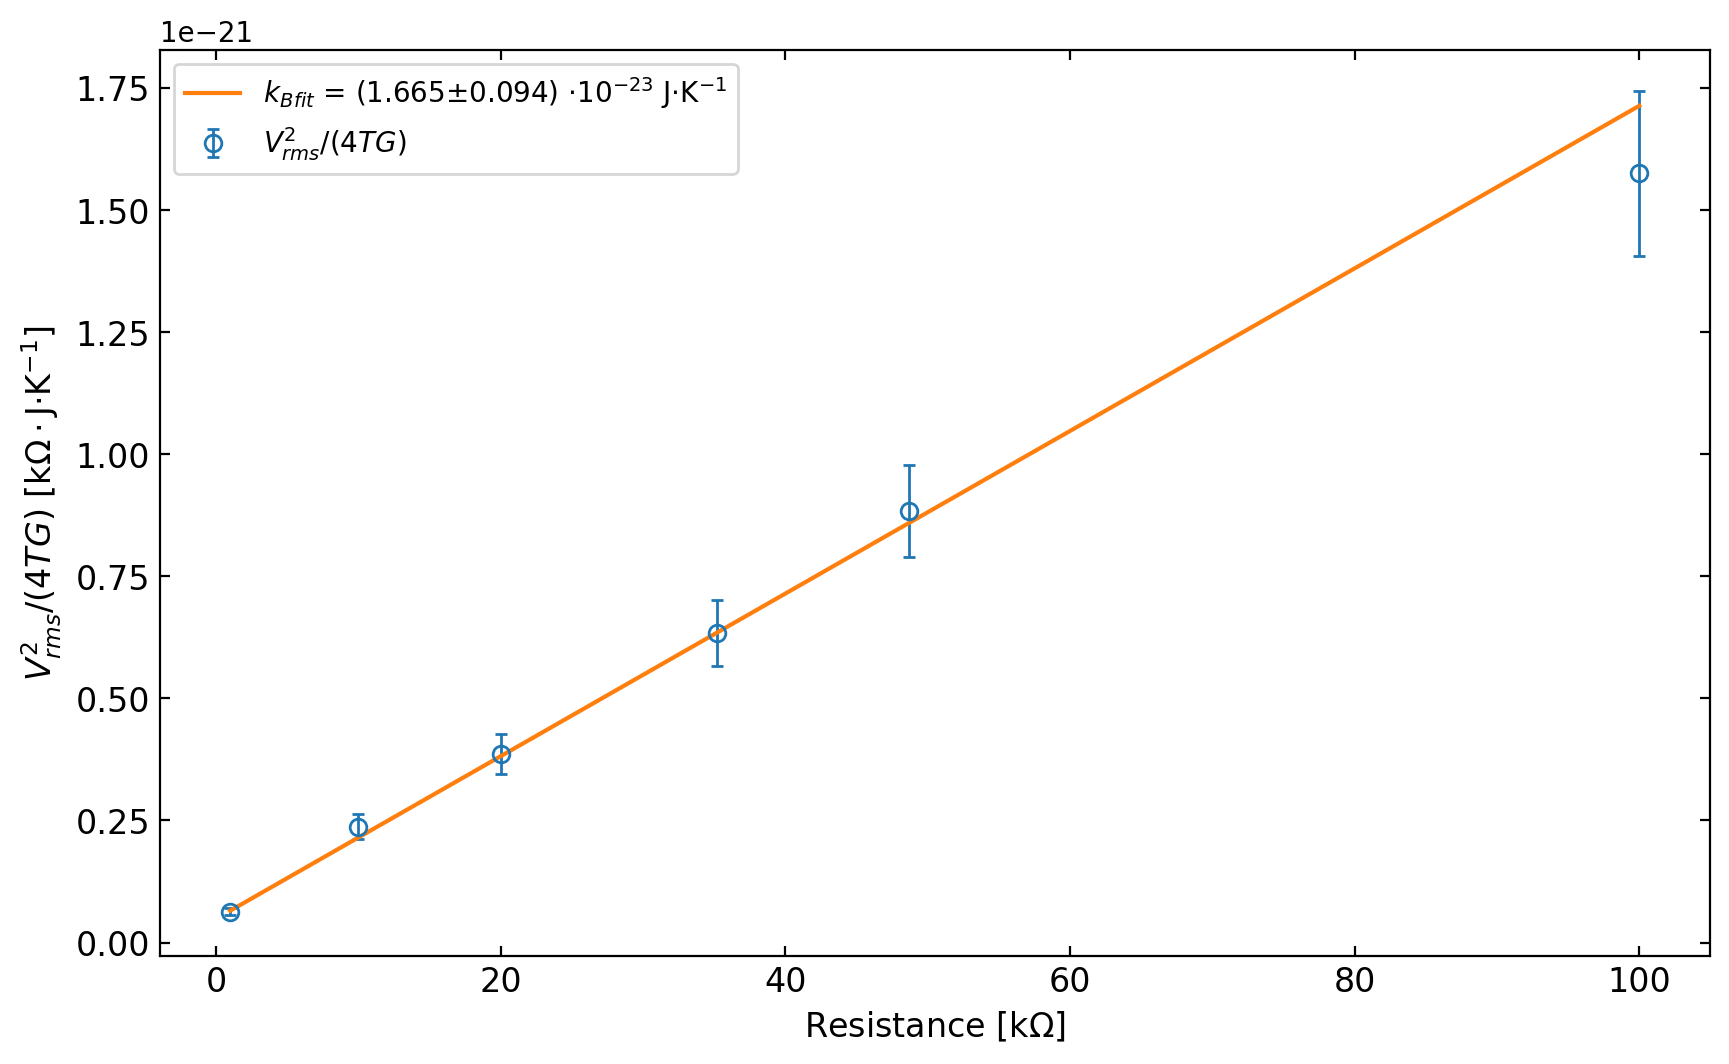
\includegraphics[width=0.8\textwidth]{images/nitro_fit.png}
    \captionof{figure}{\textbf{Analyzed Plot} - At boiling point of liquid nitrogen ($77$K), we measured Johnson noise of six different resistors again, and we performed a line fit based on ratio $V^2_{rms}/(4T G)$ versus Resistance. From this we can estimate the Boltzmann constant (proportional to slope) and its uncertainty.}
    \label{fig:boltzConst}
\end{center}

\subsection{Error Analysis}
\quad We propagate error in voltage and resistance through following equations,
\begin{equation}
    \delta g = \sqrt{\left(\pdv{g}{V_{in}} \right)^2 (\delta V_{in})^2 + \left(\pdv{g}{V_{out}} \right)^2 (\delta V_{out})^2 } 
\end{equation}
\begin{equation}
    \delta G = \sqrt{\left(\pdv{G}{g} \right)^2 (\delta g)^2 + \left(\pdv{G}{R} \right)^2 (\delta R)^2  + \left(\pdv{G}{C} \right)^2 (\delta C)^2  }
\end{equation}
\begin{equation}
    \delta T = \sqrt{\left(\pdv{T}{G} \right)^2 (\delta G)^2 + \left(\pdv{T}{R} \right)^2 (\delta R)^2 + \left(\pdv{T}{V} \right)^2 (\delta V)^2} \label{eqn:temp}
\end{equation}
\begin{equation}
    \delta k_B = \sqrt{\left(\pdv{k_B}{G} \right)^2 (\delta G)^2 + \left(\pdv{k_B}{R} \right)^2 (\delta R)^2 + \left(\pdv{k_B}{V} \right)^2 (\delta V)^2}\label{eqn:therm}
\end{equation}

For the absolute zero temperature measurement, the difference between measured result and the accepted result can be compensated by Eqn.~\ref{eqn:temp}. However, for the estimation of Boltzmann constant, the discrepancy is beyond our propagated error bars. 

We reason that the uncertainty in capacitance (C) cannot explain the upper shift of our result. Since our circuit and the coaxial cables we used are connected in series, the total effective capacitance can only decreases, which will increase the gain and decrease the slope of linear fit (measurement of $k_B$). Also, the uncertainty of resistance (R) is not large enough to explain deviation in our measurement. So we are left with the gain function and root-mean-square voltage. It is possible that the calculated gain function is offed, due to the existence of the ambient background noise of the equipment. Evidently, the background noise we measured is comparable to the un-amplified signal from noise generator. And the measurement of white noise has significant shift before and after we did other measurements (See Fig.~\ref{fig:noise_gen}). 

\begin{center}
    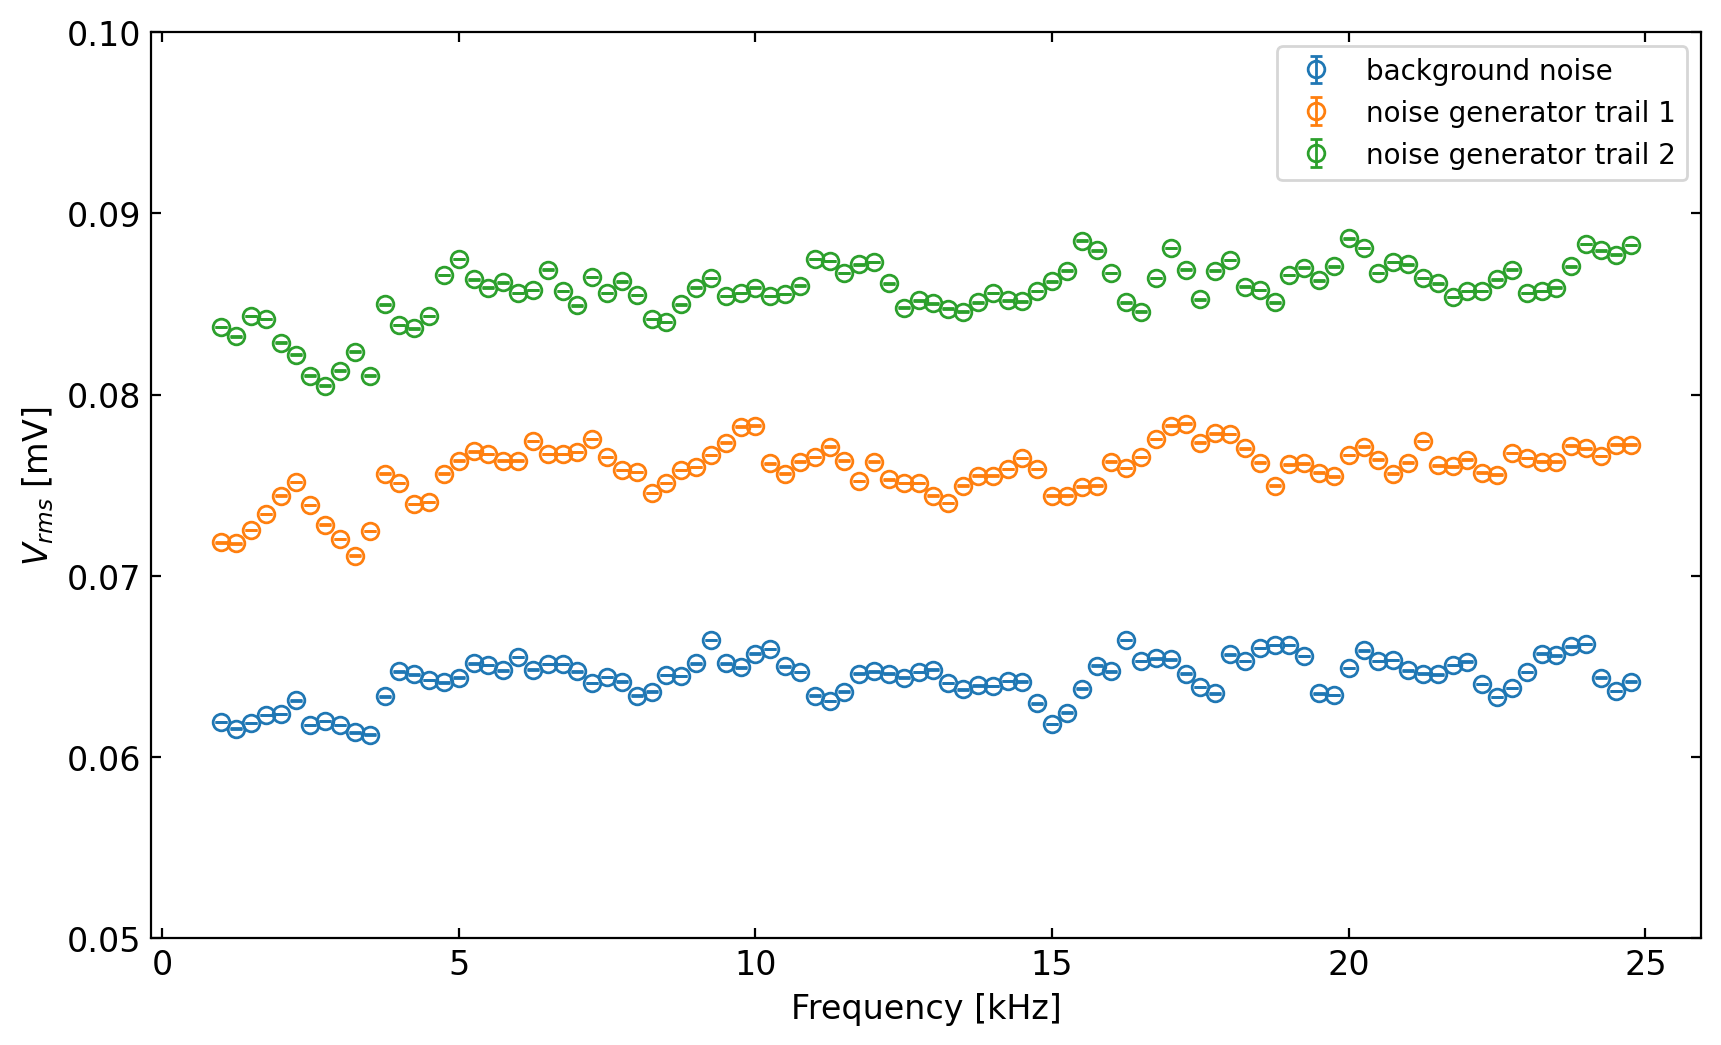
\includegraphics[width = 0.8\textwidth]{images/nosie_gen_trail.png}
    \captionof{figure}{Measurement of background noise of the spectral analyzer, and unprocessed signal from the random noise generator. We conducted trail 1 before measuring Johnson noise of the resistors, and trail 2 after we finished them. This plot suggests that our measurement of gain might not be stable, and the background noise will affect our system significantly.}\label{fig:noise_gen}
\end{center}


\section{Discussion}
\quad The Boltzmann constant we calculated are with large error compared to the accepted data. After debugging and trials, we excluded the error factors from capacitance and resistance. We concluded that the main factor that causes this large error is the gain $g(f)$. As shown in Eqn.~\ref{eqn:gain}, the gain is calculated by the division of $V_{out}$ and $V_{in}$. The value of $V_{out}$ is large enough , so we are able to measure it with a good accuracy. However, the $V_{in}$ is too small compared to the background noise, which causes the measurement not accurate and thus causes the large error we got in our calculation. Possible solution may be increasing the output voltage of the white noise generator lowering the gain of the pre-amplifier correspondingly. This way, the $V_{in}$ signal could be greater, and thus easier to separate from the background noise. 

% maybe a graph showing how close the background noise and V_in is


\end{document}
